
\documentclass[12pt, addpoints]{exam}
\usepackage[utf8]{inputenc}
\usepackage[portuguese]{babel}
\usepackage{multicol}
\usepackage{graphicx}
\usepackage{amsmath}

\setlength{\columnsep}{1cm}

\begin{document}

        
\begin{minipage}[l]{0.5\linewidth}
    \begin{flushleft}
        {\bf \Large Prova bimestral}
    \end{flushleft}
\end{minipage}
\begin{minipage}[r]{0.45\linewidth}
    \begin{flushright}
        {\bf \Large Código: XXXXX}
    \end{flushright}
\end{minipage}
\vspace{0.5cm} \hrule \vspace{0.5cm}
\begin{minipage}{0.75\linewidth}
    Aluno:
\end{minipage}
\begin{minipage}{0.20\linewidth}
    Data: 
\end{minipage}
\vspace{0.5cm} \hrule \vspace{0.5cm}

\begin{questions}
\begin{multicols*}{2}
\question[33] Durante sua trajetória uma partícula realizou um trabalho de    8.75 J. Qual foi a variação da sua energia cinética?

\begin{oneparchoices}
\choice 0.41 J\choice 3.65 J\choice 9.66 J\choice -7.96 J\choice 6.71 J\choice 4.07 J\choice 2.34 J\choice 3.68 J\choice -1.47 J\choice 8.75 J\end{oneparchoices}
\question[23] Considere uma partícula de massa    8.28 kg e velocidade    3.39 m/s. Determine a sua energia cinética.

\begin{center}
\begin{minipage}[c]{0.75\linewidth}
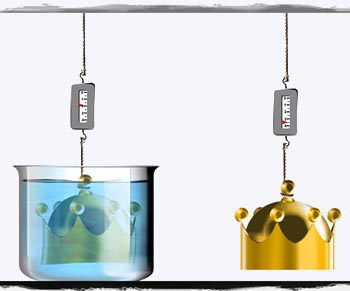
\includegraphics[width=\textwidth]{MWE001.jpg}
\end{minipage}

\end{center}
\begin{oneparchoices}
\choice 10.91 J\choice 36.95 J\choice 41.26 J\choice 47.66 J\choice 91.88 J\choice 190.88 J\choice 136.09 J\choice 423.19 J\choice 10.03 J\choice 32.13 J\end{oneparchoices}
\end{multicols*}
\end{questions}
\newpage
\begin{minipage}[l]{0.5\linewidth}
    \begin{flushleft}
        {\bf \Large Prova bimestral}
    \end{flushleft}
\end{minipage}
\begin{minipage}[r]{0.45\linewidth}
    \begin{flushright}
        {\bf \Large Código: XXXXX}
    \end{flushright}
\end{minipage}
\vspace{0.5cm} \hrule \vspace{0.5cm}
\begin{minipage}{0.75\linewidth}
    Aluno:
\end{minipage}
\begin{minipage}{0.20\linewidth}
    Data: 
\end{minipage}
\vspace{0.5cm} \hrule \vspace{0.5cm}

\begin{questions}
\begin{multicols*}{2}
\question[33] Durante sua trajetória uma partícula realizou um trabalho de   -7.39 J. Qual foi a variação da sua energia cinética?

\begin{oneparchoices}
\choice 6.35 J\choice -7.82 J\choice -7.23 J\choice -0.36 J\choice -7.39 J\choice 9.46 J\choice 5.52 J\choice -6.12 J\choice -0.66 J\choice -7.02 J\end{oneparchoices}
\question[23] Considere uma partícula de massa    4.39 kg e velocidade    1.31 m/s. Determine a sua energia cinética.

\begin{center}
\begin{minipage}[c]{0.75\linewidth}
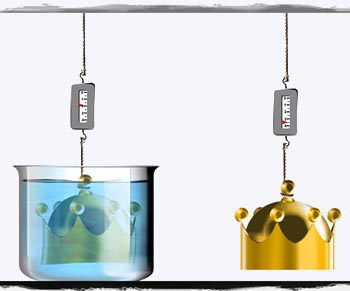
\includegraphics[width=\textwidth]{MWE001.jpg}
\end{minipage}

\end{center}
\begin{oneparchoices}
\choice 59.06 J\choice 545.32 J\choice 25.4 J\choice 456.84 J\choice 10.67 J\choice 161.39 J\choice 3.76 J\choice 320.04 J\choice 65.44 J\choice 337.2 J\end{oneparchoices}
\end{multicols*}
\end{questions}
\newpage
\end{document}
        